\newcommand{\package}{\emph}

\setcounter{chapter}{1}
\setcounter{section}{0}
\section{Simpson and Shannon index}
\subsection{a}
Since all draws are independent the probability to observe the same type in $k$ draws is simply a $k-time$ multiplication (Product Rule) of individual probabilities $pi$ (which is in essence a relative frequency of type $i$), so it it is $p^k$

Then we have to sum up such probability for each strain $i$ (additivity axiom, each draw is mutually exclusive)

So, finally

\[ D_k = \sum\limits_{i=1}^{n} p_{i}^{k} \]

We remember from our final ODE model, that after immune response reaches its equilibrium at levels $x_i^* = \frac{cv_i}{b+uv}$ and $z^* = \frac{kv}{b+uv}$ and with this values we could have a single ODE for virus load:

\[ v' = \frac{v}{b+uv} [rb -v(cpD + kq -ru)]   \]

Solution of this ODE (i.e. behavior of $v(t)$) depends on parameters and, in general, has three regimes: immediate disease, chronic infection and disease after long asymptomatic period.
A certain combination of these parameters called "antigenic diversity threshold" 

\[ D < \frac{ru-kq}{cp} \]

and it puts general equation above out of equilibrium, so causes uncontrolled grows of $v(t)$.
The only part of this equation which is changing during the course of the disease is $D$ (genetic similarity of virus). It is actually close to $1$ right after the infection and then gradually goes to smaller values (more different virus strains) till reaches its threshold value, when immune system cannot control virus anymore. From mathematical point of view increasing of  $dv/dt$ is smaller with large $D$.

\subsection{b}

For an uniform distribution of $n$ strains:
\[ H = - \sum\limits_{i=1}^{n} p_i\log(p_i) \text{ if } p_1 = p_2  = \dots = p_n \]
\[ H = -(p_i\log(p_i)+p_{i+1}\log(p_{i+1}) + \dots+p_n\log(p_n)) =  -np\log(p) = \]
\[ H = -p_i(\log p_i^n) = -np_i\log p_i \text{ and as } p_i = \frac{1}{n} \text{ for each } i \]
\[H = -n * \frac{1}{n} * \log\frac{1}{n} = - \log n^{-1} = \log n\]

For $n = 2$ :

\[ H = -p_1\log p_1 - p_2\log p_2 \]

For $p_2 = 1-p_1$ :

\[ H  = -p_1\log p_1 - (1-p_1) \log(1-p_1) \] 
\[H' = \log (1 - p_1) - \log p_1 \]

To find a maximum/minimum (stable point of $H$): $H' = 0$
\begin{align*}
0 &= -\log p_1 + \log (1-p_1)\\
\log p_1 &= \log (1-p_1)\\
p_1 &= 1-p_1\\
p_1 &= \frac{1}{2} \\
P_2 &= 1 - \frac{1}{2} = \frac{1}{2}
\end{align*}

\begin{figure}[htbp]
\centering
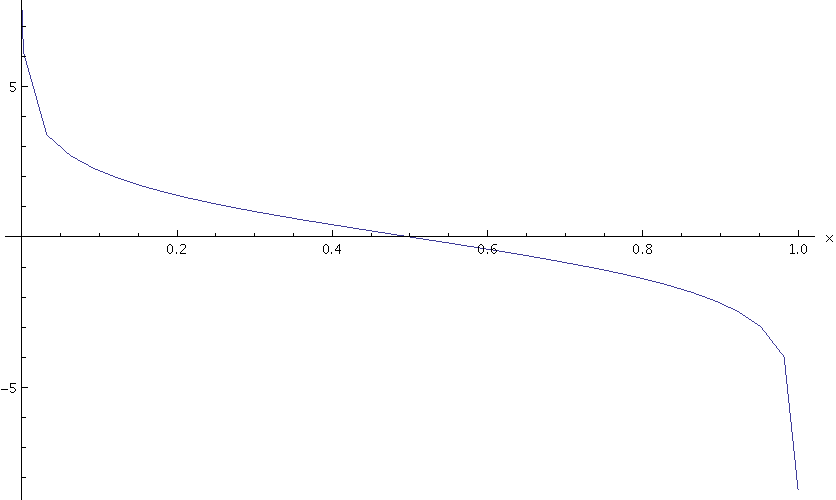
\includegraphics[scale=0.6]{./images/graph01}
\caption{H' function representation}
\label{fig:graph01}
\end{figure}

To describe wheter the point $p_1 = \frac{1}{2}$ is a maximum for $H$, we take the second derivative: $H'' < 0$:


\[  H'' = -\frac{1}{p_1\ln 10 } - \frac{1}{(1-p_1)\ln 10} = -\frac{1}{\ln 10} \left(\frac{1}{p_1}+\frac{1}{1-p_1}\right)\]

at $p_1 = \frac{1}{2}$ : $H'' = -\frac{1}{\ln 10} \left(\frac{1}{\frac{1}{2}}+\frac{1}{\frac{1}{2}}\right) = -\frac{1}{\ln 10} * 4 = -4\ln 10 < 0$

Hence, for n= 2, the uniform distribution maximizes the Shannon index.


\setcounter{chapter}{2}
\setcounter{section}{0}
\section{Epidemiological dynamics and basic reproductive ratio}
\subsection{a}
\begin{align*}
x(0) &= x_0 \\
y(0) &= y_0 \\
z(0) &= 0 \\
x' &= bN - \beta xy - bx\\
y' &= \beta xy - (b+r)y \\
z' &= ry - bZ
\end{align*}

\begin{align*}
\frac{dZ(t)}{dt} = ry(t) - bZ(t) \xRightarrow{t=0} \frac{dZ(0)}{dt} &= ry(0) - bZ(0) \\
\frac{d}{dt}(0) &= ry_0 -b(0) \\ 
0 &= ry_0 \rightarrow \boxed{ y_0 = 0}
\end{align*}

\begin{align*}
\frac{dy(t)}{dt} = \beta x(t) - (b+r)y(t) \xRightarrow{t=0} \frac{dy(0)}{dt} &= \beta x(0)y(0) - (b+r)y(0) \\
\frac{d}{dt}(0) &= \beta x_0 y_0 -(b+r)y_0  \\ 
\Aboxed{ x_0 &= \frac{b+r}{\beta}}
\end{align*}


\begin{align*}
\frac{dx(t)}{dt} = bN - \beta x(t)y - bx(t) \xRightarrow{t=0} \frac{dX(0)}{dt} &= bN - \beta x(0)y(0) - bx(0)\\
0 &= bN - bx_0  \\ 
N &= x_0 = \frac{b+r}{\beta}
\end{align*}
If $N>N_C = \frac{b+r}{\beta}$, $y$ can grow and sequentially $Z$ can grow as well.
If $y = 0$, then $x$ converges to the uninfected equilibrium $N$, while $y$ can only grow if $x$ exceeds the threshold $\frac{b+r}{\beta}$. Hence, the pathogen carrying the disease can only invade its host if this threshold is smaller than $N$. 

\[ \frac{b+r}{\beta} < N \rightarrow \frac{N}{\frac{b+r}{\beta}} > 1 \rightarrow N\frac{\beta}{b + r} > 1\]
\[ R_0 = N\frac{\beta}{b + r} \rightarrow \begin{cases} 
																	R_0 < 1 \rightarrow \text{ the parasite cannot spread}  \\
																	R_0 > 1 \rightarrow \text{ the parasite can spread and invade the host} \end{cases} \]

\subsection{b}

\begin{align*}
f(x) = \frac{dx}{dt} &= bN-\beta xy - bx \\
&\Rightarrow bN - \beta x^* y^* -bx^* = 0 \\
g(y) = \frac{dy}{dt} &= \beta xy - (b+r)y \\
&\Rightarrow \beta x^* y^* - (b+r)y^* \rightarrow x^* = \frac{b+r}{\beta}\\
h(Z) = \frac{dZ}{dt} &= ry - bZ \\
 &\Rightarrow ry^* - bZ^* = 0 \rightarrow Z^* = \frac{ry^*}{b}
\end{align*}

\[ x^* = \frac{b+r}{\beta}  = \frac{2+4}{3} = 2 \rightarrow \boxed{x^* = 2}\]
\[ bN - \beta x^* y^*-bx^* = 0 \rightarrow 2000 -6y^* -4 = 0 \rightarrow y^* = \frac{1996}{6} \rightarrow \boxed{y^*= \frac{998}{3} \approx 332.66} \]
\[ Z^* = \frac{r}{b}y^* = 2y^* = \frac{1996}{3} \rightarrow \boxed{Z^* = \frac{1996}{3} \approx  665.33333333} \]

To find stability of equilibrium $|f'(x)| < 1$:

\begin{align*}
\frac{df(x)}{dx} &= -b-\beta y &\rightarrow& 998-2 = -1000 &\rightarrow&  |f'(x)| = 1000>1 &\rightarrow& \text{ $x^*$ is not stable} \\
\frac{dg(y)}{dy} &= \beta x - (b+r) &\rightarrow& g'(y) = 6-6 = 0 &\rightarrow&  |g'(y)| < 1 &\rightarrow& \text{ $y^*$ is stable}\\
\frac{dh(Z)}{dZ} &= - b &\rightarrow& h'(Z) = -2 &\rightarrow& |h'(Z)| > 1 &\rightarrow&   \text{ $Z^*$ is not stable} \\
\end{align*}

\subsection{c}

x-null clines: $ 0 = 2000 -3xy -2x$\\
y-null clines: $ 0 = 3xy -6y$ 

Solutions:
\[x_1 = 2, y_1 = \frac{997}{3}\]
\[x_2 = \frac{2000}{3}, y_2 = 0\]

\begin{figure}[htbp]
\centering
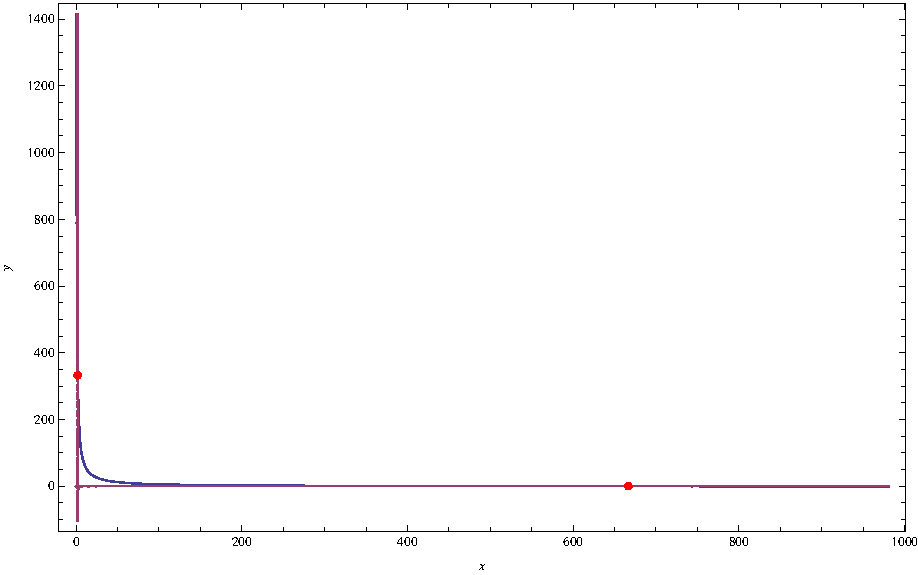
\includegraphics[scale=0.6]{./images/graph02}
\caption{Null clines graph}
\label{fig:graph02}
\end{figure}


\setcounter{chapter}{3}
\setcounter{section}{0}
\section{Random walk}
\subsection{a}
\begin{align*}
E[X(t) | X(0)  = i ] &= E[X(0) + \sum\limits_{s=1}^{t} \Delta(t) ] \\
&= E[i] + E\left[  \sum\limits_{s=1}^{t} \Delta(s) \right] \\
&= i + E \left[ \sum\limits_{s=1}^{t} \left[1 * \frac{a}{2} + 0 * (1-a) -1*\frac{a}{2}\right] \right]\\
E[X(t) | X(0)  = i ] &= i + sE(\Delta(1)) = i + s*0 = i
\end{align*}
\subsection{b}
\begin{align*}
Var[X(t) | X(0) = i] = at
Var(X(t)) &= Var(x(0) + \Delta(1) + \dots + \Delta(t))\\
&= Var(x(0) + Var(\Delta(1)) + \dots + Var(\Delta(t)))\\
&=Var(X(0)) + t*Var(\Delta(1)) = \\
\text{as }Var(\Delta(1)) &= (1-0)^2 *  \frac{a}{2} + (1-0)^2 * \frac{a}{2} + 0^2(1-a) = a\\
Var(X(t)|X(0) = i ) &= Var(i) + t* Var(\Delta(1)) = 0 + t*a = at
\end{align*}

\setcounter{chapter}{4}
\setcounter{section}{0}
\section{Neutral Moran process}
\subsection{a}

\subsection{b}

\subsection{c}

\subsection{d}

\begin{figure}[htbp]
\centering
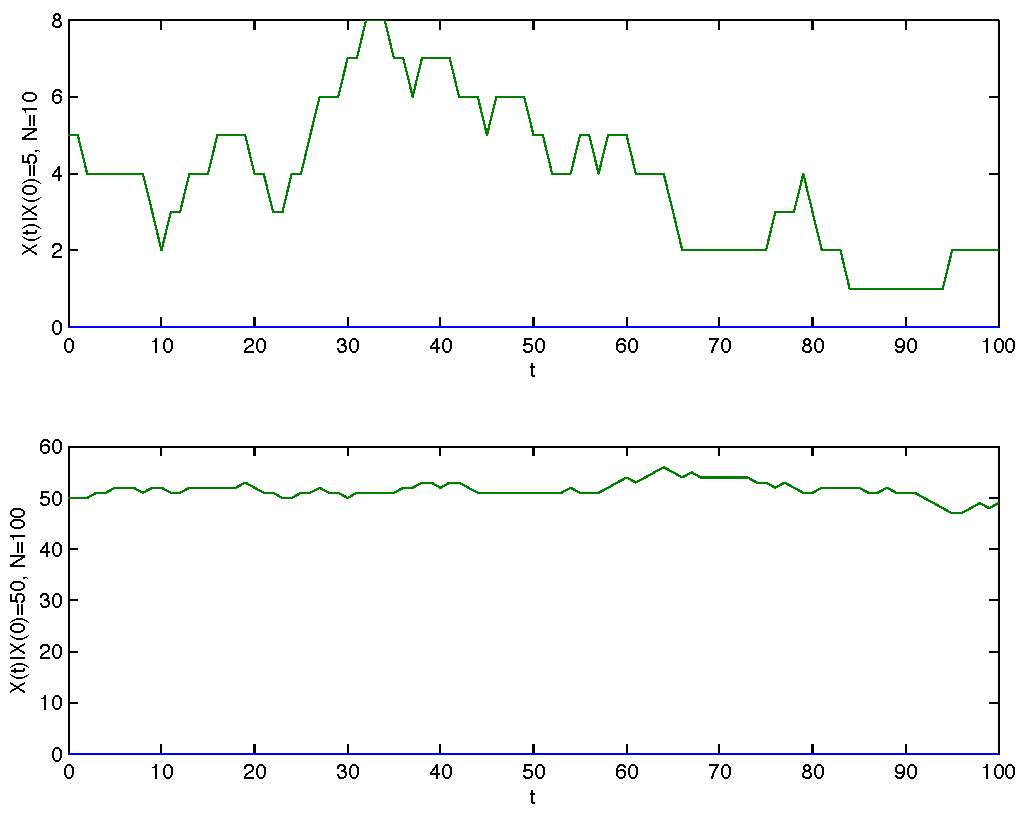
\includegraphics[scale=0.7]{./images/plot_moran}
\caption{Neutral Moran processes, with $N=10$ and $N=100$}
\label{fig:graph03}
\end{figure}

\lstinputlisting[caption={./script.m},label=lst:ev02_main]{./listing/script.m}
\lstinputlisting[caption={./moran.m},label=lst:ev02_moran]{./listing/moran.m}

\setcounter{chapter}{5}
\setcounter{section}{0}
\section{Absorption in a birth-death process}
\subsection{a}
i) $\vec{x}$ is the probability of ending up in state $N$ for $x_i \forall i=1 \dots N$\\
$t\rightarrow\inf$, $P_{ij} \rightarrow x_i \rightarrow x_i $ is unique stationary distribution. \\
The absorption probabilities are given by the right-hand eigenvector associated with the largest eigen value, which is one, because p is stochastich matrix.
\[ \vec{x}P = \vec{x} \]
\begin{align*}
x &= (x_0,\dots, x_n)^t\\
y &= x_i - x_{i-1}\\
\gamma &= \frac{\beta_{i}}{\alpha _{i}}
\end{align*}
\[p = \begin{bmatrix}
1 & 0 & 0 & \cdots & 0 & 0 & 0 \\
\beta _1 & 1-\alpha _1-\beta_1 & \alpha _1 & \cdots & 0 & 0 & 0 \\
\vdots &\vdots&\vdots&\ddots&\vdots&\vdots&\vdots\\
0 & 0 & 0 & \cdots & \beta_{N-1} & 1-\alpha_{N-1}-\beta_{N-1}&\alpha_{N-1}\\
0 & 0 & 0 & \cdots & 0 & 0 & 1 
\end{bmatrix}\]
\begin{align*}
x_0 &= 0\\
x_i &= p_{i,i-1}x_{i-1}+p_{i,i}x_i + p_{i,i+1}x_{i+1} = \beta_i x_{i-1}(1-\alpha_i - \beta_i)x_i + \alpha_i x_{i+1}\\
x_N &= 1
\end{align*}

\begin{align*}
x_i &= \beta_i x_{i-1}(1-\alpha_i - \beta_i)x_i + \alpha_i x_{i+1}\\
x_{i-1} &= \frac{(\alpha_i+\beta_i)x_i-\alpha_ix_{i+1}}{\beta_i}\\
\rightarrow y_i &= x_i - x_{i-1} = \beta_i x_{i-1} + (1-\alpha_i -\beta_i)x_i + \alpha_ix_{i+1}- \frac{(\alpha_i+\beta_i)x_i-\alpha_ix_{i+1}}{\beta_i}\\
\rightarrow y_i &= \frac{(\beta_i-\alpha_i -\beta_i)x_i+\alpha_ix_{i+1}}{\beta_i}\\
\rightarrow y_i &= \frac{\alpha_ix_{i+1} - \alpha_ix_{i}}{\beta_i} = \frac{\alpha_i}{\beta_i}(x_{i+1}-x_i) = \frac{\alpha_i}{\beta_i}y_{i+1} = \frac{1}{\gamma_i}y_{i+1}\\
\rightarrow y_{i+1} &= \gamma_iy_i
\end{align*}
ii) Show that $\sum\limits_{i=1}^{0}y_i = x_l$

\[ \sum\limits_{i=1}^{l} y_i = x_1-x_0+x_2-x_1+\dots+x_l-x_{l-1} = x_l -x_0 = x_l \rightarrow \boxed{\sum\limits_{i=1}^{l} y_i = x_l}  \]

We can conclude $\boxed{\sum\limits_{i=1}^{N} y_i = x_n = 1}$

iii) Show that $x_l = (1+ \sum\limits_{j=1}^{l-1} \prod\limits_{k=1}^{j} \gamma_K)x_1$

form point i) of this section: $y_1 = x_1$, $y_2 = \gamma_1y_1 = \gamma_1x_1$, $y_3=\gamma_2y_2 = \gamma_1\gamma_2x_1$

\[ \sum\limits_{i=1}^{l} y_i = x_1 + \gamma_1x_1 + \gamma_1\gamma_2x_1+\dots+(\gamma_1\dots\gamma_{l-1})x_1 = (1+\sum\limits_{j=1}^{l-1}\prod\limits_{k=1}^{j} \gamma_K) x_1 ) = x_l \]

\[ \rightarrow \boxed{x_l = (1+ \sum\limits_{j=1}^{l-1}\prod\limits_{k=1}^{j} \gamma_K)x_1  }  \]

We can conclude $x_N = (1+ \sum\limits_{j=1}^{l-1}\prod\limits_{k=1}^{j} \gamma_K)x_1 = 1$

\[ \rightarrow  \boxed{ x_1 = \frac{1}{ 1 + \sum\limits_{j=1}^{l-1}\prod\limits_{k=1}^{j} \gamma_K)} } \]
\[ x_i = x_1 (1+\sum\limits_{j=1}^{i-1}\prod\limits_{k=1}^{j} \gamma_K) ) \]
\[ \rightarrow  \boxed{ x_i = \frac{1+\sum\limits_{j=1}^{i-1}\prod\limits_{k=1}^{j} \gamma_K}{1+\sum\limits_{j=1}^{N-1}\prod\limits_{k=1}^{j} \gamma_K} }\]

\subsection{b}

\begin{align*}
x_i &= \frac{1+\sum\limits_{j=1}^{i-1}\prod\limits_{k=1}^{j} \gamma_K}{1+\sum\limits_{j=1}^{N-1}\prod\limits_{k=1}^{j} \gamma_K}\\
\gamma_i &= \frac{P_{i, i-1}}{P_{i,i+1}} = \frac{1}{r}
\end{align*}

\begin{align*} x_i = \frac{1+\frac{1}{r} + \frac{1}{r^2} +\frac{1}{r^3} + \dots + \frac{1}{r^{i-1}}}{1+\frac{1}{r} + \frac{1}{r^2} +\frac{1}{r^3} + \dots + \frac{1}{r^{N-1}}} = \frac{1-\frac{1}{r^i}}{1-\frac{1}{r^N}} &\rightarrow \boxed{ x_i = \frac{1-\frac{1}{r^i}}{1-\frac{1}{r^N}} }\\
&\rightarrow \boxed{ x_1 = \frac{1-\frac{1}{r}}{1-\frac{1}{r}} }
\end{align*}

\[ \lim\limits_{r\rightarrow1}  \frac{f(r)}{g(r)} = \lim\limits_{r\rightarrow1}  \frac{f'(r)}{g'(r)} =  \lim\limits_{r\rightarrow1}  \frac{\frac{1}{r^2}}{\frac{Nr^{N-1}}{r^{2N}}} = \frac{1}{N} \rightarrow \boxed{\lim\limits_{r\rightarrow1} \frac{1-\frac{1}{r}}{1-\frac{1}{r^N}} = \frac{1}{N} }   \]